% Labels inside TikZ pictures: text and mathematics in nodes, placed by
% anchors, label= and pin=, rotated, sloped along an edge, scaled, in several
% lines, in a tikz-cd diagram, inline in a paragraph and in a display. The PDF
% draws the pictures as TeX does (tex_pictures), so the capture and dvisvgm
% are tested, not taken as the reference.
\documentclass{article}
\usepackage{tikz}
\usepackage{tikz-cd}
\usetikzlibrary{arrows.meta,positioning}
\begin{document}
A paragraph before the pictures, long enough to break across lines
differently at every width the test tries, so that each picture below
moves when the text is reflowed.

\begin{center}
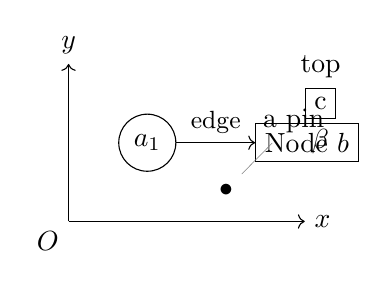
\begin{tikzpicture}
  \draw[->] (0,0) -- (3,0) node[right] {$x$};
  \draw[->] (0,0) -- (0,2) node[above] {$y$};
  \node[draw, circle] (a) at (1,1) {$a_1$};
  \node[draw, rectangle, right=of a] (b) {Node $b$};
  \draw[->] (a) -- node[above, sloped] {\small edge} (b);
  \node[below left] at (0,0) {$O$};
  \node[label=above:{top}, label=below:{$\beta$}, draw] at (3.2,1.5) {c};
  \node[pin=60:{a pin}] at (2,0.4) {$\bullet$};
\end{tikzpicture}
\end{center}
Text between two pictures, with a word or two more to fill the line.

\begin{center}
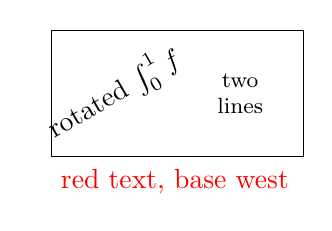
\begin{tikzpicture}[scale=0.8]
  \draw (0,0) rectangle (4,2);
  \node[rotate=30] at (1,1) {rotated $\int_0^1 f$};
  \node[align=center, font=\footnotesize] at (3,1) {two\\ lines};
  \node[anchor=base west, text=red] at (0,-0.5) {red text, base west};
\end{tikzpicture}
\qquad
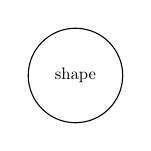
\begin{tikzpicture}[scale=0.6, every node/.style={transform shape}]
  \draw (0,0) circle (1);
  \node at (0,0) {shape};
\end{tikzpicture}
\end{center}

A commutative diagram with labelled arrows:
\[
\begin{tikzcd}
  A \arrow[r, "f"] \arrow[d, "g"'] & B \arrow[d, "h"] \\
  C \arrow[r, "k"', "\sim"] & D
\end{tikzcd}
\]
and a paragraph with a picture inline,
\tikz[baseline=(X.base)] \node[draw, circle, inner sep=1pt] (X) {$n$};,
set on the baseline of its label, and another,
\tikz \draw (0,0) -- (1,0.3) node[right] {end};, which sits on the line
as a box does, with text after both so that the line breaks move them about.
\end{document}
